\documentclass{beamer}
\usetheme{Boadilla}
\usepackage[english]{babel}
\usepackage{amsmath}
\usepackage{graphicx}
\usepackage{wrapfig}
\usepackage{color}
\usepackage{setspace}
\usepackage{multicol}
\setbeamertemplate{frametitle}{ \bf
\begin{centering} 
\insertframetitle 
\par 
\end{centering} 
} 

\newcommand\Fontvi{\fontsize{9}{9}\selectfont}
\newcommand\Fontvii{\fontsize{4}{4}\selectfont}
\newcommand\Fontv{\fontsize{11}{11}\selectfont}
\newcommand\Fontb{\fontsize{20}{20}\selectfont}
\newcommand\Fontsm{\fontsize{13}{13}\selectfont}
\newcommand\vk{\bold{k}}
\newcommand\vq{\bold{q}}
\newcommand\vx{\bold{x}}

\title{Committee Meeting}
\author[brosemeyer@physics.montana.edu]{Ben Rosemeyer \\ \small Advisor: Anton Vorontsov}
\institute[MSU]{
\includegraphics[scale=0.2]{MSUlogo.jpg}\\[0.5cm]
Funded by NSF grant DMR-0954342 \\
\includegraphics[scale=0.08]{NSFlogo.jpg}
}
\date[Committee Meeting]{\small\today}



\begin{document}
\frame{\titlepage}


\begin{frame}
\frametitle{RECAP}
\begin{center}
\includegraphics[height=0.75\textwidth, width=0.75\textwidth]{paper_shot.png}
\end{center}
\end{frame}

\begin{frame} \frametitle{RECAP}
Nodal gap has negative quasi-particle energy states when in external field
\begin{equation}
E_{\vk\sigma} = \sqrt{\xi_\vk^2 + \Delta_\vk^2} + \sigma H \quad\quad \Delta_\vk = \Delta sin(2\theta_\vk)\quad\quad \sigma = \pm 1
\end{equation}
\begin{columns}
	\begin{column}{0.5\textwidth}
    		AFM correlations which connect ("Nest") these negative/zero energy states in a particular way are enhanced
    		\begin{eqnarray}
    			\chi_{\perp}(\vq) = \sum\limits_{\vk\sigma} &\frac{A_\sigma(\vk,\vq)}{E_{\vk+\vq/2 \sigma} + E_{\vk-\vq/2 \sigma}} \\
    			 + & \frac{B_\sigma(\vk,\vq)}{E_{\vk+\vq/2 \sigma} - E_{\vk-\vq/2 \bar{\sigma}}}
    		\end{eqnarray}
    \end{column}
    \begin{column}{0.5\textwidth}
      	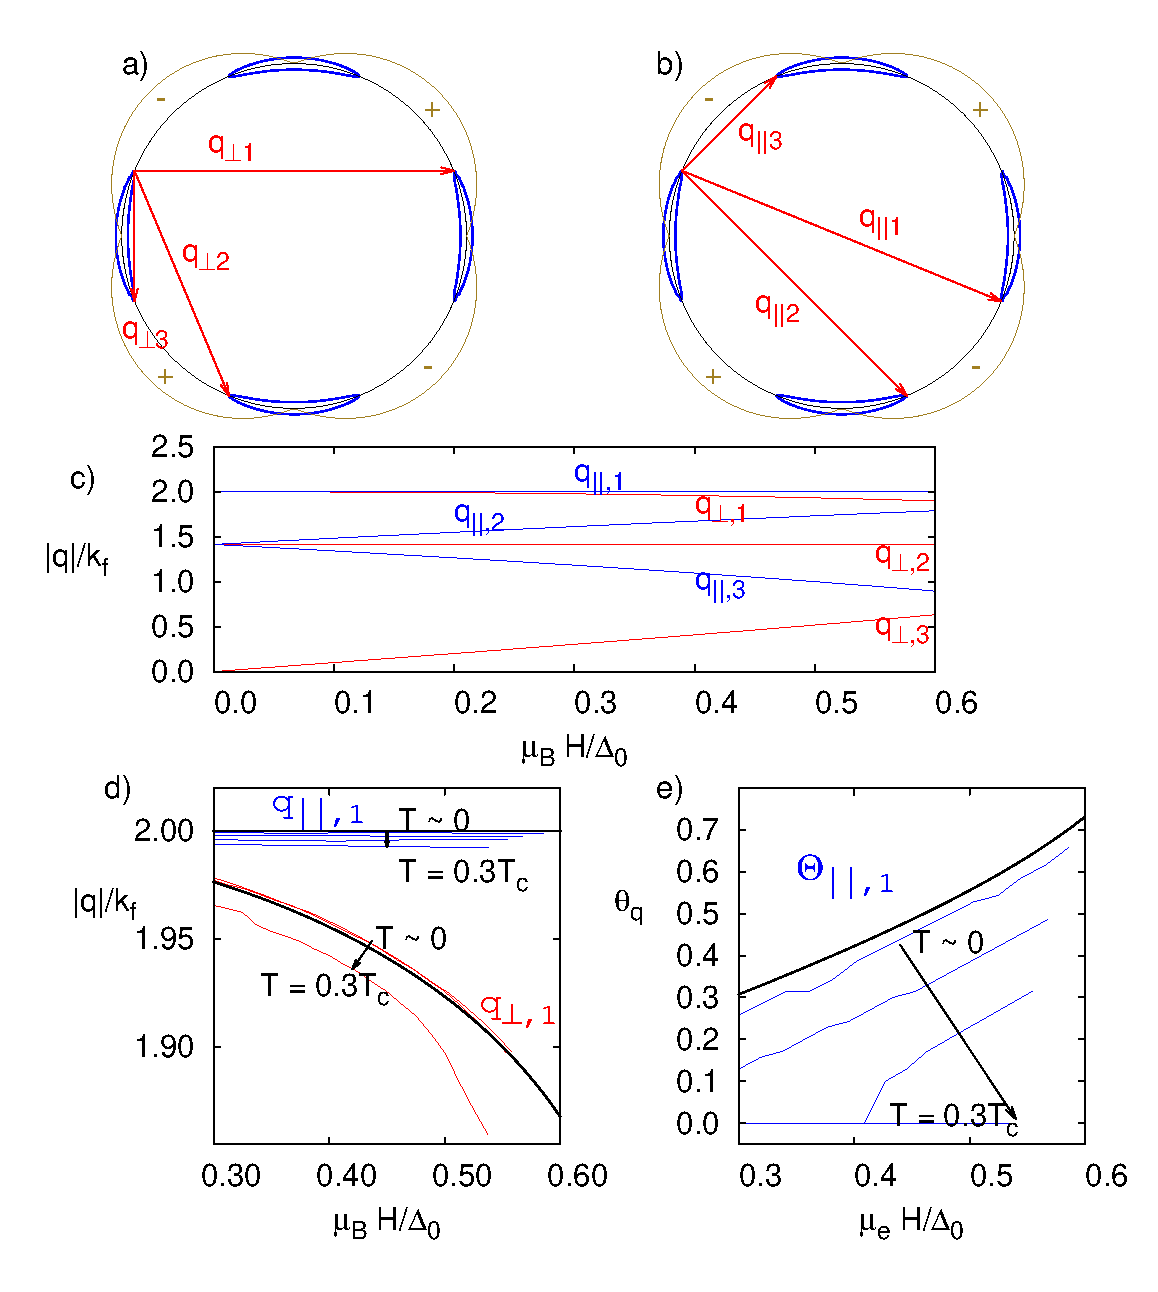
\includegraphics[scale=0.3]{Fig2.eps}
    \end{column}
  \end{columns}
\end{frame}

\begin{frame} \frametitle{RECAP}
Qualitative agreement with CeCoIn$_5$ phase diagram!
\begin{center}
		\includegraphics[scale=0.38]{Fig3.eps}
		\includegraphics[scale=0.14]{PhaseDiagramS.jpg} \\
      	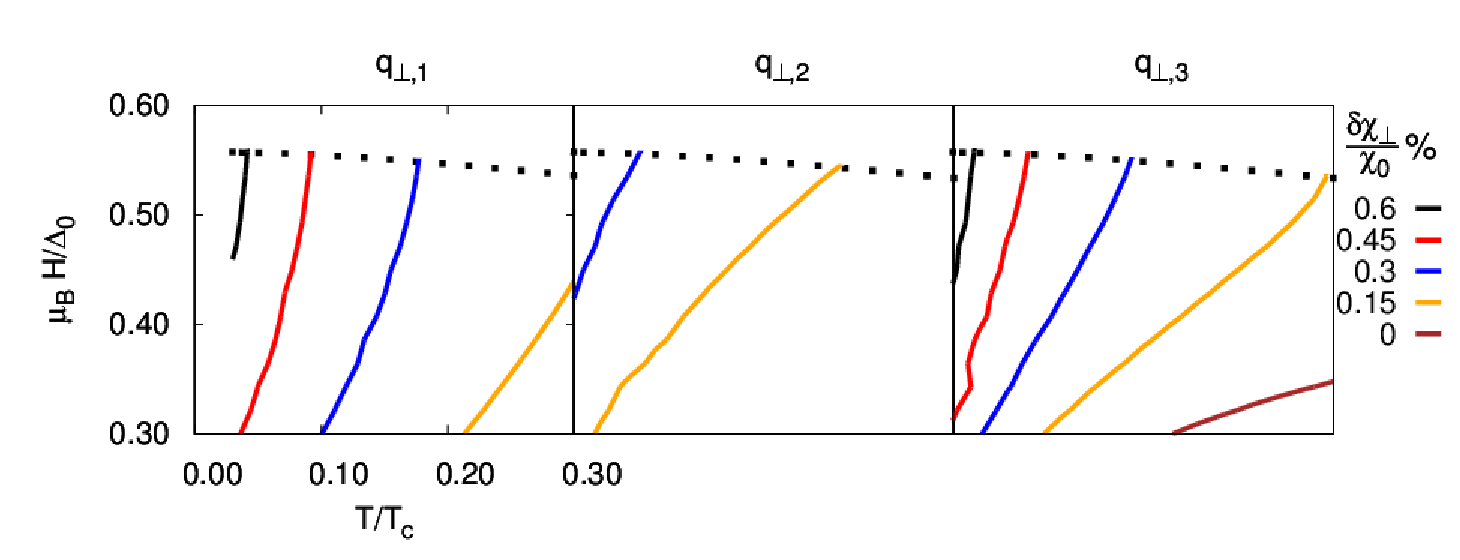
\includegraphics[scale=0.38]{Fig4.eps}
\end{center}
\end{frame}

\begin{frame} \frametitle{RECAP}
\includegraphics[scale=0.1]{surfing.JPG}
\end{frame}

\begin{frame} \frametitle{WHATS NEXT?}
INHOMOGENEOUS SUPERCONDUCTIVITY \\
- Fulde Ferrell (phase modulations) \\
- Larkin Ovchinnikov (amplitude modulations) ******** \\
- Layered Materials \\
- Josephson Junctions \\
\vspace{1cm}
-Creates quasi-particle states BELOW the gap (bound states) \\
-Increase DOS near Fermi level (whiteboard drawing)
\end{frame}

\begin{frame} \frametitle{WHATS NEXT?}
SUB-GAP STATES: \\
-momentum is no longer a good quantum number \\
 $\rightarrow$ but it's still pretty good for states far from Fermi level \\
-Need to solve Bogoliubov-de Gennes equations more carefully (whiteboard) \\
\begin{eqnarray}
 (-\delta^2_x - \mu) u_n(\vx) + \int d\vx' \Delta(\vx,\vx')v_n(\vx') = E_n u_n(\vx) \\
 -(-\delta^2_x - \mu) v_n(\vx) + \int d\vx' \Delta^*(\vx,\vx')u_n(\vx') = E_n v_n(\vx)
\end{eqnarray}
 Homogeneous: $u_n(\vx) = u_{\vk_n}e^{i\vk_n\cdot\vx}\quad \rightarrow$ Get $E_n$ from $\vk_n$  \\
 Inhomogeneous: $u_n(\vx) = \sum\limits_{\vk} u_{n\vk}e^{i\vk\cdot\vx}$ \\
 $\quad \rightarrow$ solve eigenvalue eq  for $u_{n\vk}$ and $E_n$\\
\end{frame}

\begin{frame} \frametitle{WHATS NEXT?}
\begin{eqnarray}
E_n\left( \begin{array}{cc}
. \\
u_{n\vk}  \\ 
. \\ \hline
. \\
v_{n\vk} \\
. \\ 
\end{array} \right)
=\left( \begin{array}{ccc|ccc}
. & 0 & 0 &  &  &  \\
0 & \xi_\vk & 0 & & \Delta_{\vk\vk'} & \\
0 & 0 & . &  &  &  \\ \hline
 &  &  & . & 0 & 0 \\
 & \Delta^*_{\vk\vk'} & & 0 & -\xi_\vk & 0  \\
 &  &  & 0 & 0 &  \\  \end{array} \right)
 \left( \begin{array}{cc}
. \\
u_{n\vk'}  \\ 
. \\ \hline
. \\
v_{n\vk'} \\
. \\ 
\end{array} \right)
\end{eqnarray}
\begin{eqnarray}
\Delta_{\vk\vk'} = &G[(\vk+\vk')/2] & F[\vk-\vk'] \\
   & relative\,\, FT & c.o.m.\,\, FT \\
\end{eqnarray}
-Use these states to calculate magnetic susceptibility  $\chi(\vq,\bold{R})$ \\
We started writting another paper on this but... \\
-MUST UNDERSTAND NEW QUASI-PARTICLE STATES TO SEE HOW/WHY SUSCEPTIBILITY IS ENHANCED \\
-SEE HOW NMR RELAXATION RATES ARE EFFECTED (recent paper on organic sc)
\end{frame}
\end{document}